\documentclass[10 pt,usenames,dvipsnames, oneside]{article}
\usepackage{../../../modelo-ensino-medio}



\begin{document}

\begin{center}
  \begin{minipage}[l]{3cm}

\includegraphics[width=2cm]{logo}    
\end{minipage}\hfill
\begin{minipage}[r]{.8\textwidth}
 {\Large \scshape Atividade: Clube de Esportes}  
\end{minipage}
\end{center}
\vspace{.2cm}

\ifdefined\prof
%Habilidades da BNCC
% \begin{objetivos}
% \item 
% \end{objetivos}

%Caixa do Para o Professor
\begin{goals}
%Objetivos específicos
\begin{enumerate}
\item Estudar algebricamente a resolução de sistemas a partir de determinados contextos.
\end{enumerate}

\tcblower

%Orientações e sugestões
\begin{itemize}
\item No item \titem{a)} conduza o raciocínio do aluno da seguinte maneira "Se o clube tem $120$ adultos associados, então arrecadou-se $120 \times 6 = 720$ reais com os adultos. Para o total de $1000$ reais, restam $280$ reais. Como cada criança entrou com $4$ reais, temos $280/4=70$ crianças".
\item No item \titem{b)} conduza um raciocínio análogo ao do item \titem{a)}.
\end{itemize}
\end{goals}

\bigskip
\begin{center}
{\large \scshape Atividade}
\end{center}
\fi

Um clube precisa realizar uma reforma na sua piscina, e para isso, cobrará uma taxa de cada associado. Cada adulto pagará R\$ $6{,}00$ reais e cada criança R\$ $4{,}00$. 

\begin{figure}[H]
\centering

\noindent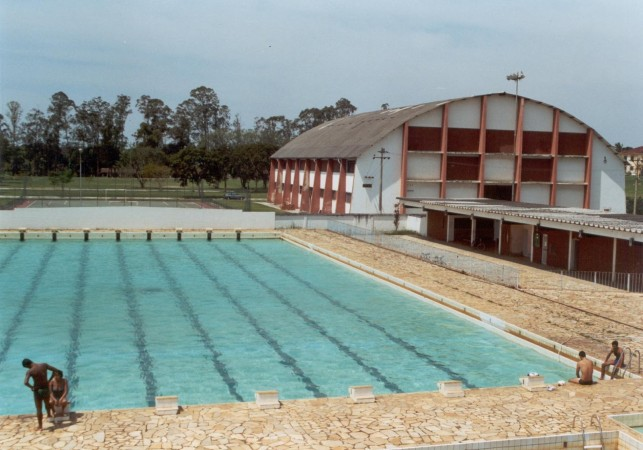
\includegraphics[width=265bp]{piscina.jpg}
\end{figure}


Sabendo que a obra está orçada em R\$ $1000{,}00$ e que o valor arrecadado foi exatamente o do preço da obra, responda:

\begin{enumerate}

\item{}
Se o clube tem $120$ adultos associados, quantos associados são crianças?

\item{}
Se forem $160$ crianças associadas, quantos serão os adultos?

\item{} 
Complete a tabela a seguir em termos de $x$ e $y$, gerando pares ordenados com essas variáveis, usando $x$ para representar o número de crianças e $y$ para representar o número de adultos.


\begin{table}[H]
\centering
\begin{tabular}{|c|c|c|}
\hline
\tcolor{N\super{o} de crianças associadas} & \tcolor{N\super{o} de adultos associados} & $\tmat{(x,y)}$ \\
\hline
$40$ &  &   \\
\hline
& $30$ & \\
\hline
& $150$ & \\
\hline
$100$ &  &  \\
\hline
$x$ &  &  \\
\hline
& $y$ & \\
\hline
\end{tabular}
\end{table}


\item{}
Escreva uma equação que relacione  o número de crianças e de adultos associados ao clube;

\item{}
Usando o GeoGebra em seu \emph{smartphone}, plote os quatro primeiros pontos dessa tabela. Você pode precisar ajustar a sua tela para conseguir visualizar esses pontos, reduzindo o zoom.
\end{enumerate}

\ifdefined\prof
\begin{solucao}

\begin{enumerate}
\item $70$ crianças.
\item $60$ adultos.
\item 
\adjustbox{valign=t}
{
\begin{tabular}{|>$e{.25\linewidth}<$|>$e{.25\linewidth}<$|>$e{.25\linewidth}<$|}
\hline
$\tcolor{N\super{o} de crianças associadas}$ & $\tcolor{N\super{o} de adultos associados}$ & \tmat{(x,y)} \tabularnewline
\hline
40 & 140 & (40,140) \tabularnewline
\hline
205 & 30 & (205,30) \tabularnewline
\hline
25 & 150 & (25,150) \tabularnewline
\hline
100 & 100 & (100,100) \tabularnewline
\hline
x & \dfrac{1000-4x}{6} & \bigg(x,\dfrac{1000-4x}{6}\bigg) \tabularnewline
\hline
\dfrac{1000-6y}{4} & y & \bigg(\dfrac{100-6y}{4},y\bigg) \tabularnewline
\hline
\end{tabular}
}
\item $4x+6y=1000$
\end{enumerate}

\end{solucao}
\fi

\end{document}